\documentclass{standalone}
\usepackage{tikz}
\usepackage{pgfplots}
\usetikzlibrary{arrows.meta}

\begin{document}

\resizebox{8cm}{8cm}{%
    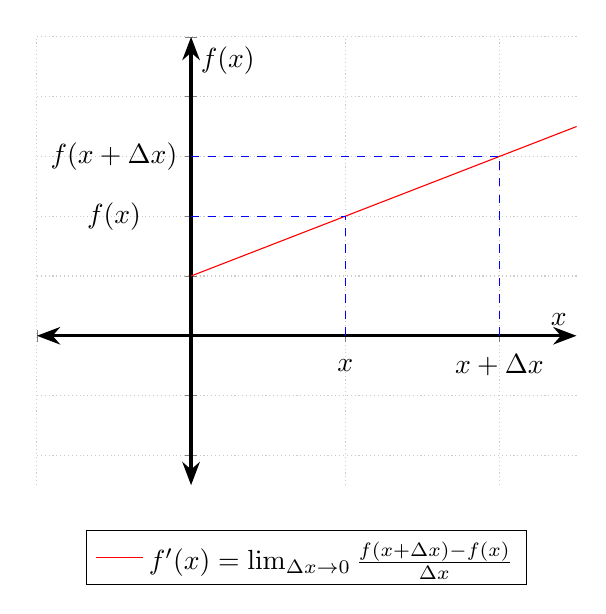
\begin{tikzpicture}
    \begin{axis}[
        title={},
        axis lines=middle,
        axis line style={Stealth-Stealth,very thick},
        xlabel=$x$,
        ylabel={$f(x)$},
        xmin=-2,xmax=5,ymin=-5,ymax=10,
        xtick distance=2,
        ytick distance=2,
        grid=major,
        grid style={thin,densely dotted,black!20},
        % No numbers on graph
        xticklabels={,,},
        yticklabels={,,},
        legend style={
            at={(0.5,-0.1)}, % Position at the center bottom
            anchor=north, % Anchor the legend at the top
            cells={anchor=west} % Align the legend entries to the left
        }
    ]
    \addplot[
        domain= 0:7,
        samples=200,
        color=red
        ]
        {x + 2};
    \addplot[
        color=blue,
        mark=none,
        dashed
        ]
        coordinates {
            (2,0)
            (2,4)
        };
    \node at (axis cs:2,-1) {$x$};
    \addplot[
        color=blue,
        mark=none,
        dashed
        ]
        coordinates {
            (4,0)
            (4,6)
        };
    \node at (axis cs:4,-1) {$x+\Delta{x}$};
    \addplot[
        color=blue,
        mark=none,
        dashed
        ]
        coordinates {
            (0,4)
            (2,4)
        };
    \node at (axis cs:-1,4) {$f(x)$};
    \addplot[
        color=blue,
        mark=none,
        dashed
        ]
        coordinates {
            (0,6)
            (4,6)
        };
    \node at (axis cs:-1,6) {$f(x+\Delta{x})$};
    \addlegendentry{$f'(x) = \lim_{{\Delta x \to 0}} \frac{f(x+\Delta x) - f(x)}{\Delta x}$}
    \end{axis}
    \end{tikzpicture}
}

\end{document}
